\documentclass{article}


\usepackage{arxiv}

\usepackage[utf8]{inputenc} 
\usepackage[T1]{fontenc}    
\usepackage{hyperref}       
\usepackage{url}
\usepackage{xcolor}            
\usepackage{booktabs}       
\usepackage{amsfonts}       
\usepackage{nicefrac}       
\usepackage{microtype}      
\usepackage{multicol}
\usepackage{mdframed}
\usepackage{physics}
\usepackage{graphicx}
\usepackage{caption}
\usepackage{nomencl}
\makenomenclature
\captionsetup[figure]{font=scriptsize}
\usepackage{siunitx}
\usepackage{tcolorbox}
\usepackage{multicol}

\begin{document}

\section*{A non-technical explanation of the main achievement of the paper}
\begin{mdframed}
\nomenclature{$QKD$}{Quantum Key Distribution}
\nomenclature{$MDIQKD$}{Measurement-Device-Independent Quantum Key Distribution}
\nomenclature{$BSM$}{Bell State Measurement}
\nomenclature{$HOM$}{Hong-Ou-Mandel}
\nomenclature{$BB84$}{Bennett Brassard 1984}
\printnomenclature
\end{mdframed}

\subsection*{Demonstrating a measurement-device-independent quantum key distribution (MDIQKD) network}


Researchers from china have successfully demonstrated a three user, four node \textit{measurement-device-independent quantum key distribution} (MDIQKD) network within the city of Hefei. Previous demonstrations of a \textit{quantum key distribution} (QKD) networks, such as by the team at moscow state university\cite{2017QuEle..47..798K} , have been proven to be successful but are vulnerable to attack by an eavesdropper (Eve). Standard QKD networks (also known as prepare and measure QKD networks) have to assume the central relays to be completely trustful. In reality this is extremely unlikely due various security loopholes associated with standard QKD networks. One such security loophole is the \textit{detection loophole}. The \textit{detection loophole} is caused by unavoidable losses in the quantum channel and  the coupling between photon source and optical fibres. Additionally losses occur due to the measurement devices finite detection efficiency. This flaw can allow Eve to perform an \textit{intercept and resend} attack, in which Eve intercepts and measures the state being transmitted and prepares a fake state to be sent to Bob. A MDIQKD network attempts to close the \textit{detection loophole} by \textcolor{red}{removing the measurement devices entirely} and instead uses a shared  central station to create entanglement-like correlations between Alice and Bob through a \textit{Bell-state measurements}(BSM). This approach is based of \textit{time-reversed entanglement based QKD}\cite{PhysRevA.54.2651} \textcolor{red}{and relies on the monogamous nature of entanglement. As Alice and Bob are connected by a fully entangled state, even if Eve completely controls the central station she can not gain any information about the cryptographic key.}

\vspace*{1mm}

Upgrading a standard QKD network to a MDIQKD network has not been attempted until now as there are two main technical challenges that arise. The first being \textit{reference frame calibration}. This refers the the real time alignment of reference frames between network users. In past attempts to achieve \textit{reference frame calibration} researcher have used additional fibre links between users. The results of this is that the demand of fibre links increases quadratically with the number of network users. This is impractical when scaling up to a city sized user populations. A solution was found by the researchers in China through a \textit{phase feedback scheme}, shown in figure 1. This allowed for a far more manageable linear scaling of fibre links with the number of network users.

\begin{figure}
  \centering 
  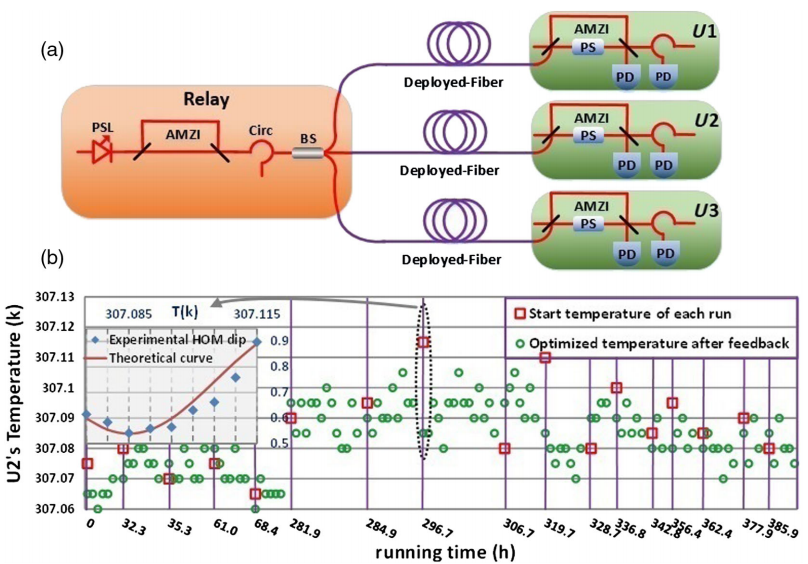
\includegraphics[width=0.7\linewidth]{phase_feedback_scheme.png}
  \caption{Phase feedback scheme\cite{PhysRevX.6.011024}.}
  \label{figure 1}
\end{figure}

The second technical challenge involves \textit{maintaining indistinguishability} between the network users. In a MDIQKD network any two users can be switched upon request. \textcolor{red}{ The new user's laser must be calibrated immediately to disallow the new and old users lasers from mixing. Mixing two users lasers would result in the timing, spectrum and polarization mode being indistinguishable between the two users.} A solution was developed using \textit{multi-user HOM interference} technology. The team believes this technology can find applications in \textit{multi-party entanglement swapping-based quantum communication} and a \textit{quantum computing cloud}.

\subsection*{Secure key rate 10 times larger than previous results}

QKD networks can be characterised by their \textit{secure key rate}.  The secure key rate gives a measure of how much secure information (measured in bits) is transmitted per second by the network. It is calculated from the networks gain rates, error rates and error correction efficiency. The secure key rate is distinct from the \textit{key rate} which only gives a measure of how much information is transmitted per second by the network. Compared to standard QKD networks the key rate for an MDIQKD network is relativity low. Under the same experimental parameters a decoy \textit{BB84 system} with a trustful relay can generate a key rate around 1000bps, \textcolor{red}{over 25 times greater than the team achieved in the MDIQKD network}. However, what a MDIQKD network lacks in key rate it makes up with security. Hence, the secure key rate achieved by the team are at least 10 times higher than previous state of the art field tests. The results are shown in figure 2.

    
\begin{figure}
  \centering 
  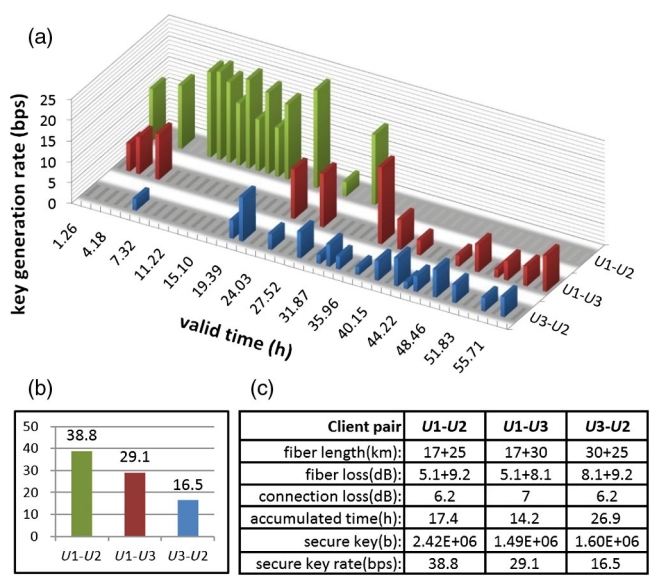
\includegraphics[width=0.7\linewidth]{Results.png}
  \caption{Secure key rate.\cite{PhysRevX.6.011024}.}
  \label{figure 2}
\end{figure}

\section*{2 or 3 “boxes” explaining, via diagrams, the key technical ideas of the experiment itself of the theory behind it}

\begin{tcolorbox}
\subsection*{Typical MDIQKD Process}

\begin{multicols}{2}

1. Alice and Bob both prepare \textcolor{red}{phase randomized weak coherent pulses (WCPs) in the four possible polarization states (\ang{0}, \ang{45}, \ang{90}, \ang{135})}.\\
2. Alice and Bob both send their states to the central relay.\\
3. \textcolor{red}{The central relay performs a bell state measurement that projects the incoming signals into a bell state}.\\
4. The relay publicly announces the bell state.\\
5. Alice and Bob then publicly announce there basis but not there associated bits.\\
6. \textcolor{red}{From the relays bell state, Alice/Bobs basis and knowing there own bit that was sent. Alice/Bob can work out the opposite parties bit that was sent}\cite{EPR}.

\columnbreak

\includegraphics[width=\linewidth]{image.png}

\end{multicols}
\end{tcolorbox}

\bibliographystyle{unsrt}  
\bibliography{references}  


\end{document}
